% SCIENTIFIC NOTATION & ORDERS OF MAGNITUDE - WORKSHEET 0 (IN-CLASS INSTRUCTION)
\documentclass[12pt, letterpaper, fleqn]{article}

% ----------------------------------------------------------
% PACKAGES
% ----------------------------------------------------------
\usepackage{graphicx}
\usepackage{xcolor}
\usepackage[most]{tcolorbox}
\usepackage{amsmath, amssymb}
\usepackage{fancyhdr}
\usepackage[utf8]{inputenc}
\usepackage[T1]{fontenc}
\usepackage{enumitem}
\usepackage{geometry}
\usepackage{tikz}
\usepackage{needspace}
\usepackage{multicol}

\usetikzlibrary{arrows.meta, calc, positioning}

% ----------------------------------------------------------
% PAGE SETUP
% ----------------------------------------------------------
\usepackage{times}
\geometry{letterpaper, top=1.25in, bottom=1.25in, marginpar=0.5in}

% ----------------------------------------------------------
% HEADER / FOOTER
% ----------------------------------------------------------
\newcommand{\logowidth}{3cm}
\setlength{\headheight}{20pt}
\setlength{\footskip}{40pt}

\pagestyle{fancy}
\fancyhf{}
\fancyhead[C]{\small\bfseries Scientific Notation \& Orders of Magnitude}
\fancyfoot[L]{\raisebox{2pt}{
\includegraphics[width=\logowidth]{../kss.png}}}
\fancyfoot[C]{\thepage}
\fancyfoot[R]{8.20.0}

\renewcommand{\footrulewidth}{0.2pt}

% ----------------------------------------------------------
% THEME COLOR
% ----------------------------------------------------------
\definecolor{customteal}{HTML}{2fbdb9}

% ----------------------------------------------------------
% HELPER MACROS
% ----------------------------------------------------------
\newcommand{\blank}{\underline{\hspace{2.2cm}}}
\newcommand{\blanklong}{\underline{\hspace{6.5cm}}}
\newcommand{\blankshorter}{\underline{\hspace{1.5cm}}}

% ----------------------------------------------------------
% DOCUMENT
% ----------------------------------------------------------
\begin{document}

\textbf{Name:} \underline{\hspace{5cm}}
\hfill
\textbf{Date:} \underline{\hspace{3cm}}\\

% ==========================================================
% SECTION 1: FOUNDATION
% ==========================================================
\begin{tcolorbox}[colback=customteal!20]
    \large\textcolor{black}{\textbf{Foundation: Scientific Notation}}
\end{tcolorbox}

\vspace{3mm}

\noindent
\textbf{Scientific Notation} is a shorthand way of writing very large or very small numbers. It has two parts: a number between $1$ and $10$, multiplied by a power of $10$.

\begin{itemize}
    \item \textbf{Format:} $a \times 10^n$, where $1 \le a < 10$ and $n$ is an integer.
    \item \textbf{Large Numbers:} Have a \textbf{positive} exponent. E.g., $3,000,000 = 3 \times 10^6$. The exponent tells you how many places the decimal moved to the left.
    \item \textbf{Small Numbers:} Have a \textbf{negative} exponent. E.g., $0.00045 = 4.5 \times 10^{-4}$. The exponent tells you how many places the decimal moved to the right.
\end{itemize}

\vspace{4mm}

% ==========================================================
% VISUAL REPRESENTATION
% ==========================================================
\begin{tcolorbox}[colback=white, colframe=black!25, boxrule=0.6pt, arc=4mm, left=6mm, right=6mm, top=5mm, bottom=5mm]

\textbf{Visual Representation: Moving the Decimal}

\medskip

\begin{center}
\begin{tikzpicture}[scale=0.9]

% Example 1: Large Number
\node[font=\Large] at (2, 2) {$4$};
\node[font=\Large] at (2.5, 2) {$2$};
\node[font=\Large] at (3, 2) {$0$};
\node[font=\Large] at (3.5, 2) {$0$};
\node[font=\Large] at (4, 2) {$0$};
\node[font=\Large] at (4.5, 2) {$0$};
\filldraw[red] (4.8, 1.9) circle (1.5pt);

\draw[->, thick, red] (4.8, 1.7) to[bend left=45] (4.3, 1.7);
\draw[->, thick, red] (4.3, 1.7) to[bend left=45] (3.8, 1.7);
\draw[->, thick, red] (3.8, 1.7) to[bend left=45] (3.3, 1.7);
\draw[->, thick, red] (3.3, 1.7) to[bend left=45] (2.8, 1.7);
\draw[->, thick, red] (2.8, 1.7) to[bend left=45] (2.3, 1.7);

\node at (3.5, 0.8) {$4.2 \times 10^{\mathbf{5}}$ (Moved left 5 times)};

% Example 2: Small Number
\begin{scope}[shift={(7,0)}]
\node[font=\Large] at (2, 2) {$0$};
\filldraw[red] (2.2, 1.9) circle (1.5pt);
\node[font=\Large] at (2.5, 2) {$0$};
\node[font=\Large] at (3, 2) {$0$};
\node[font=\Large] at (3.5, 2) {$0$};
\node[font=\Large] at (4, 2) {$8$};
\node[font=\Large] at (4.5, 2) {$1$};

\draw[->, thick, blue] (2.2, 1.7) to[bend right=45] (2.7, 1.7);
\draw[->, thick, blue] (2.7, 1.7) to[bend right=45] (3.2, 1.7);
\draw[->, thick, blue] (3.2, 1.7) to[bend right=45] (3.7, 1.7);
\draw[->, thick, blue] (3.7, 1.7) to[bend right=45] (4.2, 1.7);

\node at (3.5, 0.8) {$8.1 \times 10^{\mathbf{-4}}$ (Moved right 4 times)};
\end{scope}

\end{tikzpicture}
\end{center}

\end{tcolorbox}

\vspace{4mm}

\newpage

% ==========================================================
% WORKED EXAMPLES
% ==========================================================
\begin{tcolorbox}[colback=customteal!20]
\large\textcolor{black}{\textbf{Converting to Standard Form}}
\end{tcolorbox}

\noindent
To convert back to a normal number (Standard Form), do the opposite! If the exponent is positive, make the number bigger (move decimal right). If it's negative, make it smaller (move decimal left).

\vspace{3mm}

\begin{tcolorbox}[colback=white, colframe=black!25, boxrule=0.6pt, arc=4mm, left=6mm, right=6mm, top=5mm, bottom=5mm]

\textbf{Worked Example 1: Standard Form}

\medskip

\textbf{Problem A:} Convert $3.7 \times 10^4$ to standard form.

\medskip

\textbf{Solution A:} The exponent is $+4$. Move the decimal $4$ places to the \textbf{right} to make it a big number. Add zeroes as placeholders.
\[ 3.7 \rightarrow 37000. \implies \textbf{37,000} \]

\medskip
\hrule
\medskip

\textbf{Problem B:} Convert $5 \times 10^{-3}$ to standard form.

\medskip

\textbf{Solution B:} The exponent is $-3$. The decimal is invisibly after the $5$. Move it $3$ places to the \textbf{left} to make it a small number.
\[ 5. \rightarrow .005 \implies \textbf{0.005} \]

\end{tcolorbox}

\vspace{4mm}

% ==========================================================
% PRACTICE 1
% ==========================================================
\begin{tcolorbox}[colback=white!15, colframe=black, boxrule=1.5pt, arc=4mm, left=6mm, right=6mm, top=5mm, bottom=5mm]

\textbf{Guided Practice: Basic Operations}

\medskip

\noindent
\textbf{1.} Write $8,500,000$ in scientific notation. \blanklong
\vspace{1.5cm}

\noindent
\textbf{2.} Write $0.000072$ in scientific notation. \blanklong
\vspace{1.5cm}

\noindent
\textbf{3.} Convert $9.1 \times 10^5$ to standard form. \blanklong
\vspace{1.5cm}

\noindent
\textbf{4.} Convert $2.4 \times 10^{-2}$ to standard form. \blanklong
\vspace{1.5cm}

\end{tcolorbox}

\newpage

% ==========================================================
% THINKING PROBLEM
% ==========================================================
\begin{tcolorbox}[colback=customteal!20]
\large\textcolor{black}{\textbf{Deeper Thinking: Comparing Magnitudes}}
\end{tcolorbox}

\vspace{3mm}

\begin{tcolorbox}[colback=white!15, colframe=black, boxrule=1.5pt, arc=4mm, left=6mm, right=6mm, top=5mm, bottom=5mm]

\textbf{Deeper Thinking Problem 1: Order of Magnitude}

\medskip

\noindent
When you want to know how many times larger one number is than another, you can compare their powers of $10$. Each increase of $1$ in the exponent means the number is $10$ times bigger.

\vspace{5mm}

\noindent
\textbf{a)} The population of a large country is roughly $3 \times 10^8$. The population of a small town is roughly $3 \times 10^4$. How many times larger is the country's population than the town's? Show your calculation using exponent rules.

\vspace{4cm}

\noindent
\textbf{b)} A red blood cell is about $8 \times 10^{-6}$ meters wide. A grain of sand is about $2 \times 10^{-3}$ meters wide. Approximately how many red blood cells would fit across a grain of sand?

\vspace{4cm}

\end{tcolorbox}

\end{document}
